\documentclass{standalone}

\usepackage{circuitikz}

\begin{document}

% INT_AY20_MP3_L17_Fig04_Exponential_graphs.png

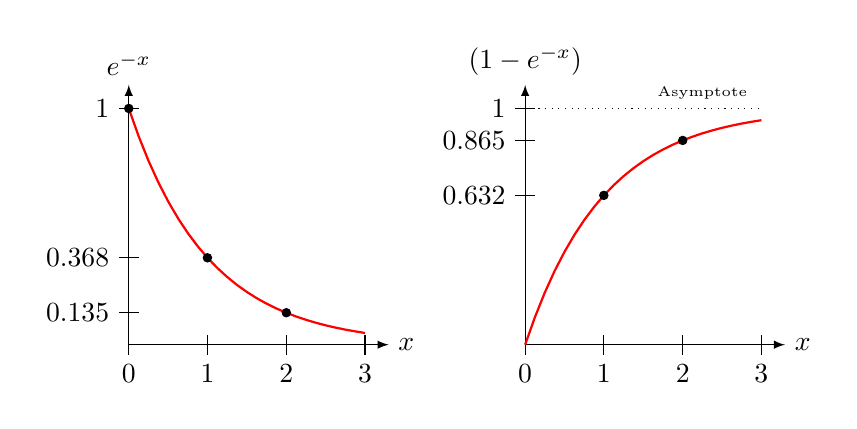
\begin{tikzpicture}

	% Definitions
	
	\def\X{3}	% Horizontal distance scale
	\def\Y{3}	% Vertical distance scale
	
	\matrix[column sep = 0.125 cm]{

	% Axes
	
	\draw [<->, > = latex] (0, 1.1 * \Y) node [above] {$e^{-x}$} -- (0, 0) -- (1.1 * \X, 0) node [right] {$x$};
	
	% Actual graph
	
	\draw [thick, red] plot[variable = \r, domain = 0:\X] (\r, {\Y * exp(-3 * \r / \X)});
	
	% Mark points on graph line
	
	\filldraw (0, \Y) circle (1.5 pt);
	\filldraw (0.333 * \X, {\Y * exp(-1)}) circle (1.5 pt);
	\filldraw (0.667 * \X, {\Y * exp(-2)}) circle (1.5 pt);
	
	% Marks on axes
	
	\draw (-0.125, \Y) node [left] {1} -- (0.125, \Y);
	\draw (-0.125, {\Y * exp(-1)}) node [left] {0.368} -- (0.125, {\Y * exp(-1)});
	\draw (-0.125, {\Y * exp(-2)}) node [left] {0.135} -- (0.125, {\Y * exp(-2)});
	
	\draw (0, 0) -- (0, -0.125) node [below] {0};
	\draw (0.333 * \X, 0.125) -- (0.333 * \X, -0.125) node [below] {1};
	\draw (0.667 * \X, 0.125) -- (0.667 * \X, -0.125) node [below] {2};
	\draw (\X, 0.125) -- (\X, -0.125) node [below] {3};

	&

	% Axes
	
	\draw [<->, > = latex] (0, 1.1 * \Y) node [above] {$(1 - e^{-x})$} -- (0, 0) -- (1.1 * \X, 0) node [right] {$x$};
	
	% Actual graph
	
	\draw [thick, red] plot[variable = \r, domain = 0:\X] (\r, {\Y * (1 - exp(-3 * \r / \X) )});
	
	% Mark points on graph line + asymptote
	
	\filldraw (0.333 * \X, {\Y * (1 -  exp(-1) )}) circle (1.5 pt);
	\filldraw (0.667 * \X, {\Y * (1 - exp(-2) )}) circle (1.5 pt);
	\draw [dotted] (0, \Y) -- node [near end, above, font = \tiny] {Asymptote} (\X, \Y);
	
	% Marks on axes
	
	\draw (-0.125, \Y) node [left] {1} -- (0.125, \Y);
	\draw (-0.125, {\Y * (1 - exp(-1) )}) node [left] {0.632} -- (0.125, {\Y * (1 - exp(-1) )});
	\draw (-0.125, {\Y * (1 - exp(-2) )}) node [left] {0.865} -- (0.125, {\Y * (1 - exp(-2) )});
	
	\draw (0, 0) -- (0, -0.125) node [below] {0};
	\draw (0.333 * \X, 0.125) -- (0.333 * \X, -0.125) node [below] {1};
	\draw (0.667 * \X, 0.125) -- (0.667 * \X, -0.125) node [below] {2};
	\draw (\X, 0.125) -- (\X, -0.125) node [below] {3};
	
	\\
	};

\end{tikzpicture}

\end{document}